\chapter{总结与展望}

\section{全文总结}

随着云计算的兴起和通用处理器性能提升的放缓,基于 FPGA 的可编程网卡在数据中心被广泛部署。
本文提出,不同于传统的计算加速,FPGA 在数据中心应当成为一等公民。
具体地,本文提出了一个基于可编程网卡的高性能数据中心系统,即利用可编程网卡提高云计算中计算、网络和存储节点的性能,并降低成本。

首先,我们提出用基于 FPGA 的可编程网卡加速云计算中的虚拟网络功能。为了简化编程,提出了首个适用于高速网络数据包处理、基于高级语言的 FPGA 编程框架。相比传统基于CPU的网络功能,把吞吐量提高了10倍,延迟降低到1/10,还为每个计算节点节约了1/5的CPU核。

其次,我们提出用可编程网卡加速远程数据结构访问。我们以内存键值存储系统为例,在服务器端绕过CPU,用网卡直接访问主机内存,实现了10倍于CPU的吞吐量和微秒级的延迟,是首个单机性能达到10亿次每秒的通用键值存储系统。

最后,为了降低软件网络协议栈的开销,我们提出一个软硬件结合的套接字网络协议栈,与现有应用程序完全兼容,并能实现接近硬件极限的吞吐量和延迟,解决了长期以来通用协议栈性能较低、专用协议栈兼容性较差的矛盾。

\section{未来工作展望}

本节简述若干进行中或正在筹划阶段的研究项目,作为未来的工作展望。

\subsection{基于片上系统的可编程网卡}
\label{future:progammable_nic}


\begin{figure}[htbp]
	\centering
	\subfloat[本文使用的 Catapult 可编程网卡。]{
		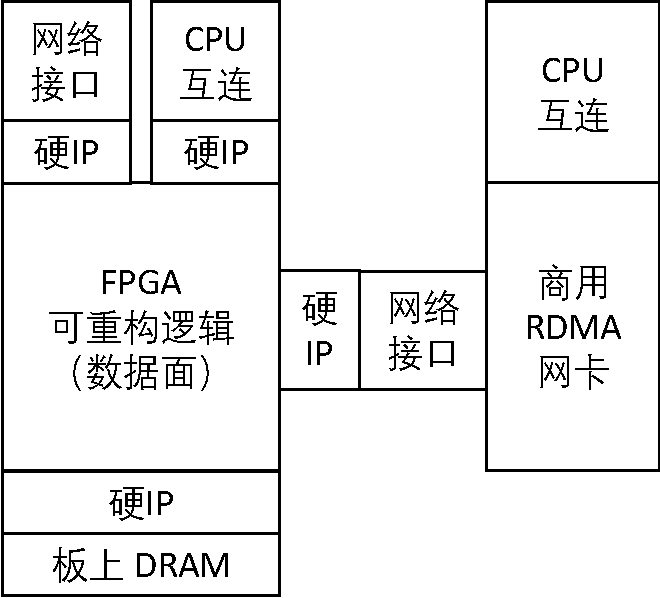
\includegraphics[width=0.4\textwidth]{figures/smartnic-current.pdf}
		\label{conclusion:fig:smartnic-current}
	}
	\hspace{0.05\textwidth}
	\subfloat[未来的片上系统。]{
		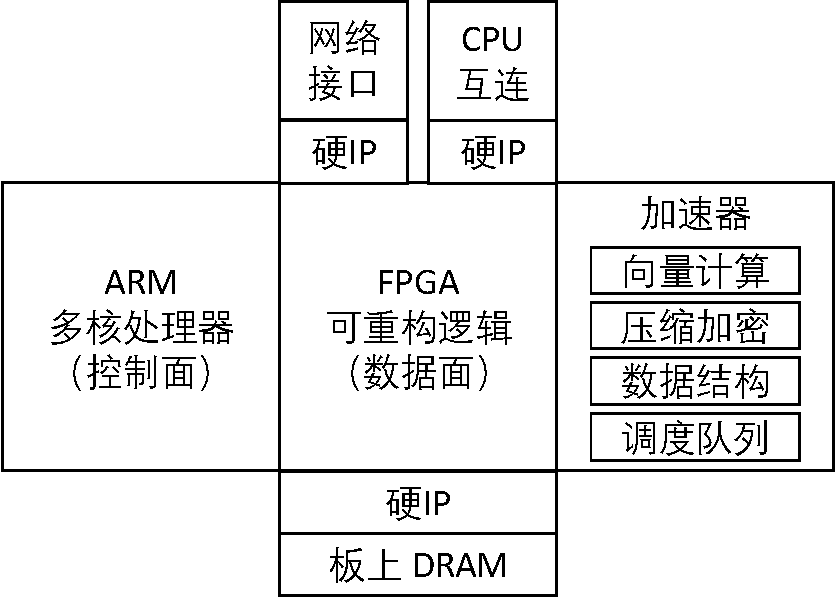
\includegraphics[width=0.5\textwidth]{figures/smartnic-soc.pdf}
		\label{conclusion:fig:smartnic-soc}
	}
	\caption{可编程网卡结构的比较。}
\end{figure}

本文使用了图 \ref{conclusion:fig:smartnic-current} 所示的 Catapult 可编程网卡。这种架构有三个局限性。
首先,现有的商用 RDMA 网卡当并发连接数较多时,性能会急剧下降 \cite{mprdma}。我们希望利用第 \ref{chapter:kvdirect} 章可扩放键值存储的技术,在 FPGA 可重构逻辑中实现 RDMA 硬件传输协议,实现高并发连接数下的高性能。这已经在第 \ref{socksdirect:sec:discussion} 节讨论过。
其次,FPGA 只适合加速数据面,控制面仍然留在主机 CPU 上。尽管它的计算量不大,但为了性能隔离,计算节点仍然需要预留少量 CPU 核用于控制面处理。第 \ref{chapter:intro} 章已经指出,即使预留一个物理 CPU 核也是相当昂贵的。为此,我们希望在可编程网卡中加入 ARM 多核处理器,用于实现控制面,从而完全消除主机 CPU 上的虚拟化开销。ARM 多核处理器的成本为数十美元,远低于一个物理 CPU 核的成本。
最后,一些类型的工作负载在 FPGA 内实现的效率不是很高,应当固化在 ASIC 加速器中。第一类是深度学习和机器学习中的向量操作、加密解密操作等计算密集型操作。例如,Intel QuickAssist 加速卡 \cite{intel-qat} 基于 ASIC 的 RSA 非对称加密比第 \ref{chapter:clicknp} 章基于 FPGA 的实现,吞吐量约高 10 倍;基于 ASIC 的 LZ77 压缩算法比我们基于 FPGA 的实现,吞吐量也高一个数量级。所用 ASIC 和 FPGA 芯片的功耗、面积和制程都接近。
第二类是常见数据结构和调度队列。基于内容寻址内存(Content-Addressable Memory,CAM)的查找表是哈希表、乱序执行引擎、缓存、模糊匹配表等多种常见数据结构的必要组件。CAM 在 ASIC 中可以用三态门实现,而在 FPGA 中实现的效率较低 \cite{wong2011comparing}。
此外,优先队列(可用移位寄存器序列或堆实现)、轮转(round-robin)调度队列、考虑依赖关系的乱序执行调度器、定时器等结构在很多应用中广泛使用,从而可以借鉴网络处理器(Network Processor)的架构,将这些通用结构硬化,让 FPGA 可重构逻辑专注于定制化计算和灵活互连。

因此,我们希望未来的可编程网卡使用如图 \ref{conclusion:fig:smartnic-soc} 所示的片上系统架构。
位于片上系统中心的 FPGA 不仅提供了可编程性和计算能力,也可以灵活互连和组合片上的各种计算加速器,组建定制化的内存层次结构,还可以灵活互连主机内外的各种硬件设备,组成数据中心智能互连(intelligent fabric)。
由于硬件平台的限制,本文尚未实现这样的硬件架构,这将作为未来的研究工作。

\subsection{基于可编程交换机的全序消息散播}


在有任意延迟的网络中,消息不能保证按照一致的顺序被投递。例如,分布式数据库的多个分片向多个副本发送日志。每个副本可能以不同的顺序收到各个分片的日志。如果不加特殊处理,这种不一致的顺序可能破坏数据一致性。解决这个问题的方案经常引入同步开销,并使分布式系统的设计复杂化。

全序通信提供了一种抽象,保证不同的接收端按照一致的顺序处理来自发送端的消息。
全序(但不可靠)地传递一组消息可以简化和加速很多分布式应用,例如减少多版本并发控制(MVCC)协议中的冲突,加速分布式共识协议,实现无中心瓶颈的可扩放日志复制(replication),提早检测 TCP 尾丢包,降低散播-汇聚(scatter-gather)模式远程过程调用(RPC)的尾延迟。

自从分布式系统研究的兴起,全序广播和多播问题就吸引了大量的研究。然而,现有方案受限于可扩放性或效率。一类研究工作利用逻辑上中心化的协调,例如中心化的序列号发生器,或者在发送端或接收端之间传递的令牌。因此,这样的系统难以扩放。另一类研究工作用完全分布式的协调,例如在接收端开始处理消息之前交换时间戳。这导致额外的网络通信开销和延迟,降低系统效率。此外,多播的语义还有一个限制,即所有接收者必须收到相同的消息。

作为正在进行的工作,我们提出全序消息散播(Total-Order Message Scattering,TOMS)原语。
我们把多播原语泛化到消息散射原语。消息散射是一种一个主机同时发送一组(可能不同的)消息给多个主机的通信原语。消息散射在分布式系统中很常见。例如在分布式存储中,一个客户端把元数据写到一个存储站点,把数据写到另一个存储站点;与此同时,另一个客户端并发地读取它们。元数据和数据间的一致性要求这些操作被原子地散射到两个存储站点。
全序消息散播在数据中心网络中一对多地散射一组消息,并保持可线性化的顺序,每条消息至多被投递一次。

我们寻找一种在数据中心环境中为分布式系统提供的可扩放且高效的可靠有序通信方案。在数据中心环境中,网络拓扑是规则的,交换机一般有较好的可编程性。
全序消息散播把工作分配给每个交换机和终端服务器,从而实现了高可扩放性。
我们的核心设计原则是把顺序信息的处理与消息转发分离开来。
为了得到顺序信息,我们利用可编程交换机,在网络中汇聚顺序信息,这形成了系统的 ``控制面''。
在 ``数据面'' 上,全序消息散播像往常一样转发消息,并在接收端缓冲并重排收到的消息。
发送端给散播的每组消息打上递增的时间戳,而接收端需要按照时间戳的顺序向应用投递消息。
控制面的顺序信息为接收端提供了 ``在此之后收到的消息都晚于某个时间戳'' 的屏障(barrier),使其可以按照时间戳顺序投递消息。


全序消息散播可以使用 P4 可编程交换机或商用交换机实现。
我们的初步测试表明,全序消息散播可以实现高性能,同时具有低 CPU 和网络开销。
作为案例研究,全序消息散播在 YCSB+T 负载下提升了分布式原子键值操作吞吐量的 50 倍(相比锁),在强竞争的 TPC-C 支付事务中实现了 100 倍于标准 MVCC 算法的可扩放性。

本研究的初步工作已经由我们的合作者左格非发表在 ACM SOSP 2017 学生研究竞赛(SRC)上。

\subsection{结合在线事务、批量和流式处理的响应式数据库}

现代大数据处理主要有在线事务处理(OLTP)、批量处理(batch processing)和流式处理(stream processing)三种范式。在线事务处理用于需要较快响应时间、较强一致性的事务,一般每个事务只涉及数据集的一小部分,且更新操作频繁。批量处理主要用于离线数据分析,其特点是数据量和计算量都很大。流式处理适用于需要高实时性的分析任务,可以针对数据的改变增量地更新状态并输出结果。

传统上,大数据处理系统一般使用 lambda 架构,即在线事务处理作为批量处理和流式处理的数据源,其产生的数据更新分别同步到批量处理部分和流式处理部分。批量处理部分定期重新计算结果,而流式处理部分根据上次的批量处理结果和流式输入的更新数据来持续更新输出。最后,批量处理部分和流式处理部分的输出被合并起来,输出给用户。首先,lambda 架构需要数据分析人员显式把数据分成在线、批量和流式三部分,分别编写处理程序,并将结果归并,开发较复杂,且容易导致不一致。其次,lambda 架构中的流式处理可能依赖上次批量处理的结果,批量处理延迟可能导致结果的不准确性,而这种延迟在性能上不一定必要。

近年来,在同一个数据库中结合在线事务处理(OLTP)和离线数据分析处理(OLAP)事务的 HTAP(Hybrid Tranactional and Analytical Processing)数据库开始流行。HTAP 数据库解决了从在线事务处理到批量处理分析的延迟问题,但仍然不支持流式处理。用户需要显式重新运行查询来获取更新后的批量处理结果,而且处理是基于查询开始时的数据库状态,不能反映数据库的实时状态。学术界提出的 DBToaster 等响应式数据库结合了在线事务处理和流式处理,但所有中间结果都被缓存和增量处理,其中的开销是很大的。例如,一些类型的批量处理难以增量更新,性能上比较合理的做法是允许一定的数据更新延迟。

我们正在设计和实现 ReactDB,一个同时高效支持在线事务处理、离线数据分析和流式处理的响应式数据库系统。ReactDB 的响应式体现在三方面。首先,每个存储过程事务都对其他并行事务的更新操作是响应式的。基本表的更新被同步到运行着的离线数据分析和流式处理事务。这些正在运行的事务保存适当的中间状态,并增量更新之。因此,每个事务都天然地在事务完成时间被序列化,也就是存储过程事务的查询结果反映了数据库的实时状态。流式处理事务则被认为是持续运行的,能够把数据库增量更新对查询结果的改变实时报告给用户。

其次,事务处理的计算流图的 ``推'' 和 ``拉'' 是响应式的。在数据库内部的计算流图中,传统数据库的每个算子都是 ``拉'' 模式的,也就是每次用户需要查询结果时,就重新执行计算流图;而流式处理和响应式数据库中,每个算子都是 ``推'' 模式的,也就是每次基础表的数据有更新时,都会更新并保存所有中间算子的结果,直到更新最终查询结果,不论用户是否需要实时的更新。我们提出根据用户对更新时效的需求来动态调整计算流图中每个算子的 ``推'' 和 ``拉'' 模式,以及 ``推'' 的频率。

最后,在 ReactDB 中,物理数据存储结构与索引是响应于数据访问模式的。
我们把基础表的数据更新日志作为数据源,而基于行、列的数据存储结构都是缓存,为点查询和分析性查询分别优化。索引也被认为是缓存。视图和分析型查询的中间结果也可能被缓存下来。
我们需要根据数据的访问模式来调整缓存与否的选择,因为缓存可以加速读操作,但对写操作增加了负担。

\subsection{通用分布式应用的透明高效容错}

分布式应用的高可用性,即容错(fault tolerance)是很重要的。
很多现有的请求处理和批量处理系统可以简化分布式应用的容错编程。
这些程序通常需要程序员把组昂泰显式地从计算中分离,并把状态存储到一个容错存储系统中。
然而,很多现有应用(如 Node.js,Memcached 和 Tensorflow 中的 Python 逻辑)并不原生支持容错。此外,容错编程框架通常比不容错的版本性能低。
作为未来工作,我们希望解决通用分布式应用程序的透明和高效容错的挑战。
具体来说,挑战分为进程迁移、确定性重放和分布式快照三个方面。

首先,在不同层次上的容错存在着权衡。
在体系结构层次上的容错需要定制化硬件。
在虚拟机层次上的容错认为所有网络通信都是双向的(因为有数据传输和 ACK 确认报文),并且不能发现诸如进程间通信的高层次语义。
系统调用层次上的容错需要对操作系统内核的修改以实现进程迁移,例如,从源主机把进程状态提取出来,并注入到目的主机里。
Linux 系统中的进程迁移较为复杂,因为来自不同进程的状态混杂在一个宏内核中。
而 Unikernel 方法不能支持很多现有的进程间通信机制。
为此,我们采用本文第 \ref{chapter:socksdirect} 章的 SocksDirect 架构,设计了一个分布式的用户态运行库操作系统,与现有 Linux 应用程序编程接口兼容。
因此,进程的内存快照同时获得了运行库和应用程序的状态,同时保留了高层语义,便于优化。

第二,状态机复制(State Machine Replication,SMR)和快照重放是实现容错的两种主要方法。 SMR 至少需要两台主机才能执行完全相同的应用程序,从而引入 CPU 开销。基于快照的系统通常在两个相邻快照之间的间隔期间缓冲应用程序的输出,因为当主机发生故障时,系统无法保证自上次快照以来的确定性执行。这种所谓的输出提交问题为透明容错系统引入了显着的请求服务延迟。或者,记录应用程序的所有非确定性事件仍然会产生很大的开销。为此,FTLinux 根据其最近的执行历史来预测应用程序的非确定性事件。如果预测正确,则应用程序继续。否则,FTLinux 会等待很短的时间来实现预测,因为许多不确定性源于微小的时间波动。超时时,FTLinux 记录错误预测的事件。

第三,透明容错机制需要在不暂停整个系统的情况下拍摄分布式应用程序的快照。一致的快照算法要求所有主机以相同的速度拍摄快照,并在任何主机发生故障时同时回滚。这种全局同步的行为与容错的目标相矛盾,容错需要系统在主机发生故障时继续提供对延迟敏感的请求。为了在不中断健康主机的情况下从单个主机故障中恢复,FTLinux暂时将每个主机的输出保存在发送方主机上,并从其邻居中保存的输出中恢复主机的输入。要从多个主机的同时故障中恢复,通信图中的每个强连接组件都需要一致的快照。 FTLinux根据库OS中的信息为每个快照间隔构造此图。此外,如果主机的快照开销高于记录其输入和输出(例如,内存密集型计算),我们可以通过记录其邻居中的通信来降低主机的快照频率。

作为未来工作,我们计划在运行Linux内核的商用服务器上设计并实现了FTLinux。 我们使用请求服务和批处理应用程序来评估FTLinux。 对于请求服务应用程序,如Nginx,Node.js,Memcached和SQLite,FTLinux可以实现透明的容错,可忽略不计的请求延迟和CPU开销。 一台主机发生故障不会影响系统的其余部分,故障主机可以快速恢复。 根据我们的性能预估,对于诸如GraphX,Apache Storm和Tensorflow等批处理应用程序,FTLinux还表现出低CPU开销和快速恢复。 值得注意的是,按照估计的性能,FTLinux的容错开销和恢复速度甚至优于GraphX,Apache Storm和Tensorflow的内置容错机制。


\subsection{基于交互测试的网络应用数据面自动生成}

为了提升网络应用的性能、降低 CPU 开销,数据中心引入了可编程交换机和网卡以卸载虚拟化网络功能、传输协议、键值存储、分布式一致性协议等。与通用处理器相比,可编程交换机和可编程网卡的资源较少,支持的编程模型也较为受限。
为此,开发者通常把一个网络功能分割成处理通常情况数据包的数据面和处理其余情况的控制面。数据面功能在一个数据包处理语言(如 P4)中实现,并卸载到硬件。

为网络应用卸载而编写数据包处理程序需要很多劳动。首先,即使拥有协议说明书或源代码,开发者仍然需要阅读上千页的文档或代码,进而发现哪一部分是常用功能。其次,很多实现与协议说明书之间存在细微的区别,因而开发者经常需要检查数据包的抓包记录,手工反向工程出特定于一个实现的行为。

作为未来工作,我们提出 P4Coder,一个能自动学习指定网络应用的行为,从而自动生成数据面参考代码的系统。
开发者只需设计一些简单的数据面的测试用例,并运行指定的网络应用。
P4Coder 将捕获输入和输出的数据包,并搜索一个数据包程序来对指定的输入测试用例产生测试得到的输出。
显然,通过测试用例并不意味着程序能在其他输入的情况下正确地泛化,因此 P4Coder 生成的代码只能作为开发者的参考,开发者可以在其基础上补充特殊情况处理的细节。尽管如此,P4Coder 生成的参考程序可以帮助开发者理解协议在通常情况下的工作方式,节约大量开发时间。

为了尽可能泛化测试用例,我们使用生成测试(generate and test)的方法来观察指定应用的行为。为了在可能的无穷多种可以生成指定输出的程序中选定一种,我们使用奥卡姆剃刀准则,选择具有最小描述长度的程序。当存在多个描述长度相同的程序时,P4Coder 生成判定性测试用例来决定正确的那个,或者报告用户。

一般意义上,通过例子生成程序被认为是困难的,由于巨大的搜索空间和理论上不可判定的停机问题。幸运的是,可以被卸载到硬件的数据包程序通常是比较简单的。商用可编程交换机和网卡并不支持循环和递归,因此不存在停机问题的判定难题。此外,对于每个持久化状态,每个数据包在数据面上只允许一次读写操作。而且,从数据包输入到输出的逻辑深度被硬件的流水线深度所限制。这些限制极大地降低了程序的搜索空间。更重要的是,为了减小搜索空间,P4Coder 可以主动生成测试用例,以消除一些可能的搜索方向。

我们预计,P4Coder 可以生成一系列可以在 P4 编程语言中实现的应用程序数据面。
例如,P4Coder 可以学习数据包数据域(packet field)的映射(如输入源 IP 对应输出目的 IP),变换(如减小 TTL)和约束(如 IP 版本号必须为 4)。P4Coder 可以推理出数据包数据域之间的映射(如根据 IP 版本号 4 或者 6 来选择不同的解析方式),以及变长数据包域(如 TCP 选项)。P4Coder 允许用户定义难以学习的定制化变换函数(如加密协议)。P4Coder 还可以生成涉及可变状态的数据包处理状态机(如数据包计数器和 TCP 连接状态)。在有合适的参考程序和测试用例的情况下,像 Paxos 这样复杂的有状态协议也可以被合成。

\subsection{硬件加速应用程序的微秒级延迟隐藏}

使用定制化硬件加速应用程序上的 CPU 处理时,原有的 CPU 软件处理逻辑被替换成了向加速器发送命令、等待加速器处理和从加速器接收结果三个步骤。在等待加速器处理期间,CPU 线程被阻塞。传统上,开发者一般采用增加更多线程的方式隐藏加速器处理延迟,也就是让操作系统在加速器处理期间切换到其他线程进行处理。然而,随着数据中心加速器性能的提高和加速任务粒度的降低,一些加速任务的执行时间只有数微秒至数十微秒。类似地,访问外部服务的远程过程调用(RPC)网络延迟也从之前的数毫秒降低到数微秒至数十微秒。操作系统切换线程调度也需要 3 至 5 微秒,几乎与加速任务的执行时间和远程过程调用的网络延迟相当。这就意味着在等待期间切换到其他线程并不经济,让 CPU 在当前线程上等待加速任务完成可能是更好的做法。但是,这也就意味着等待期间 CPU 时间的浪费,在一定程度上影响了定制化硬件加速器节约 CPU 的效果。

为此,我们计划从编译的角度出发,实现应用程序的微秒级延迟隐藏。
我们有两个主要的观察:首先,应用程序可能有多个互相不依赖的硬件加速任务需要处理,因此可能挖掘出这些不依赖的加速任务,进行并发处理。
其次,很多应用程序是事件驱动的,也就是在一个永久循环里依次处理到来的事件。不同的事件处理之间可能没有依赖关系,这时就可以暂时挂起正在被处理的事件,去处理下一个不相关的事件。

这两种延迟隐藏方案的难度在于 ``依赖关系'' 的判断。在函数式编程语言中,纯函数之间的依赖关系比较容易判断。但在大多数开发者通常使用的过程式编程语言中,内存是共享的,很多代码之间都存在依赖。例如,创建对象时需要分配内存,影响内存布局,因此从严格意义上讲,任意两个对象的创建顺序都是有依赖的。再如,两个远程过程调用是否存在依赖,往往取决于其语义。因此,问题的核心挑战是由开发者指明哪些依赖事实上是不必要的。

我们提出 ``async'' 修饰器,允许开发者指定一个函数可以被异步执行。async 函数内部可以使用 wait 调用来注册事件、释放 CPU 并在事件成立时唤醒(例如等待加速器或远程过程调用的返回)。可被异步执行的函数执行过程中不会被打断(除非调用了 wait,或有可被异步执行的子例程),因此不必担心可重入问题。每个 async 函数的执行用协程(coroutine)实现。进一步地,我们提出 ``async pure'' 修饰器,允许开发者指定一个函数不仅可以被异步执行,还没有任何副作用,这样就可以推测执行,即在执行的条件尚未确定时就执行之,而无需担心其产生不可撤回的副作用。

例如,把无状态计算卸载到加速器、只读的远程过程调用、打开文件是 async pure 函数。而执行写操作的远程过程调用、处理一个事件的例程是一般的 async 函数。如果 async 函数之间存在逻辑依赖关系,例如同一个用户发起的不同事件需要按顺序依次处理,那么可以为每个用户设置一个锁,在事件处理开始时加锁并在结束后解锁。锁使用 wait 调用实现,因此开销很小。

\subsection{基于可编程网卡的低性能损失内存解聚}

内存解聚(Memory Disaggregation)指的是计算机的 CPU 可以自由而透明地高效共享远程计算机的内存,这样可以大大增加内存的利用率,降低云计算平台的成本。
尽管目前数据中心网络的性能远低于 CPU 访问主机内存的性能,幸运的是,利用内存访问的局部性,如果一部分热数据仍在本地,剩余的数据通过远程访问,则远程内存的带宽和延迟要求能比本地内存大大降低。加州大学伯克利分校的研究指出,要把内存解聚后的系统性能与全部使用本地内存的差距控制在 5\% 以内,带宽需要达到40 Gbps,端到端往返延迟需要不超过3 至 5微秒,这是目前的数据中心网络可以达到的。

目前的大多数内存解聚系统(如 Infiniswap)的研究采用页面换入换出的方式。首先,页面换入换出需要经过操作系统内核,每换入一个页面需要增加约 2.5 微秒的内核开销,而我们允许的端到端访问延迟只有 3 至 5 微秒。其次,解聚到远程存储的内存一般是冷数据,这些数据的访问粒度可能小于一般为 4 KB 的页面大小,因此传输一整个页面不仅浪费网络带宽,也增加了延迟。最后,页面换入换出的决策在软件上进行,难以准确统计每个页面的访问频率。

为此,我们提出基于可编程网卡的内存解聚。我们使用直接内存映射取代页面换入换出,从而避免了操作系统内核的开销,也把内存访问的粒度从 4 KB 的页面降低到 64 字节的缓存行。本地与远程内存仍然是以页面为单位,依靠页表维护映射关系。可编程网卡可以统计每个页面的远程内存访问,从而及时把热数据迁移到本地内存,避免长期影响性能。

基于现有 CPU 和 PCIe 体系结构实现基于直接内存映射的内存解聚存在一系列技术挑战。幸运的是,由于非易失性内存(NVM)的兴起,CPU 厂商也意识到了同样的问题。因此,我们期待随着 CCIX 等主机内互连协议的实现,直接内存映射的可编程网卡与 CPU 之间将达到更好的吞吐量和延迟,并且直接内存映射区域可以像主机内存一样运行所有指令。


\subsection{数据中心内的无状态硬件传输协议}

以 RDMA 为例的硬件传输协议在数据中心越来越流行,因其具有低延迟、高吞吐量和低 CPU 开销的特点。然而,现在的 RDMA 网卡的内存有限,从而存储连接状态的空间受限。
当连接的数量超过内存容量时,网卡需要把连接状态通过 PCIe 换出到主机内存,导致性能损失。

我们计划探索基于硬件的无状态传输协议。
核心的方法是让连接状态在两个终端服务器之间来回乒乓。
为了让一个连接可以有多个并发数据包,我们将连接状态划分成多个不共享状态的逻辑线程,每个线程被分配一组特定序列号的数据包。
我们开发了线程分叉、限速和合并的一系列技术,仿真了基于窗口和显式拥塞通知(ECN)的拥塞控制算法。
为了支持丢包恢复,我们考虑到数据中心网络中的丢包较为稀少,设计了一个基于时间片的所有连接共享的单次丢包检测器,使选择性重传所需的存储空间与每个往返延迟(RTT)中期望的丢包数量成正比。
当丢包数量超出网卡的处理能力时,接收端 CPU 将被通知来恢复丢包。

我们计划在可编程网卡内设计和实现无连接状态的 RDMA、TCP 和 TLS 传输协议。
相比传统有连接状态的版本,这些传输协议消耗了较少的网络带宽和较低的 CPU 开销。
仿真实验表明,无状态连接和传统有状态连接可以公平地共享网络瓶颈的带宽。
在网卡的内存大小恒定的前提下,对于高并发场景,我们的无状态基于硬件的 TLS 传输协议达到了有状态传输协议性能的 100 倍。



\subsection{基于 FPGA 的 PCIe 设备透明调试器}

数据中心服务器承载着越来越多的 PCIe 设备,如 GPU、NVMe SSD、网卡、加速卡和 FPGA 等。为了 PCIe 设备之间高吞吐量和低延迟的通信,GPU-Direct、NVMe over Fabrics 等技术开始流行。然而,很多 PCIe 设备只能跟 CPU 上的设备驱动程序通信,其 PCIe 寄存器和 DMA 接口很复杂,且可能没有文档。为了在 PCIe 上抓包和调试 PCIe 协议的实现,开发者往往需要昂贵的 物理层 PCIe 协议分析仪(价值 25 万美元左右)。协议分析仪需要实验室环境,难以在生产环境中动态调试。而且,协议分析仪无法修改 PCIe 数据包,也没有足够的可编程性来从大量的流量数据中发现异常或统计规律。

在这个未来的工作中,我们利用基于 FPGA 的 PCIe 卡,设计和实现了一个透明 PCIe 传输层协议(TLP)调试器。PCIe 调试器抓取 PCIe 设备和 CPU 之间的通信数据包。这项工作的挑战在于,由于 PCIe 的物理拓扑和路由是固定的,不可能在 PCIe 上实施与局域网中的 ARP 类似的攻击。
然而,我们可以欺骗设备驱动程序,把 PCIe 流量重定向到 PCIe 调试器。
根据请求的发起方,我们把 PCIe 和 CPU 之间的通信分成两类。

第一类是 CPU 发起的内存映射 I/O(MMIO)操作。这类操作中,CPU 访问 PCIe 基址寄存器(BAR)指向的内存区域。驱动程序从操作系统内核例程中获得 BAR 地址,因此我们可以修改该操作系统内核例程,返回 PCIe 调试器的地址,而非设备本身的地址。然后我们在 PCIe 调试器中建立地址映射,使 CPU 的内存映射 I/O 操作传输到 PCIe 调试器,PCIe 调试器作为代理再把请求发送给目标设备。

第二类是设备发起的 DMA 操作,用以访问主机内存。表面上看来,我们没有办法预知设备会访问哪个内存地址。然而,良定义的设备应当只访问驱动程序分配给该设备的地址。在 Linux 中,有两种设备驱动程序获取可 DMA 内存区域及其物理地址的方法。我们可以对这两种操作系统例程分别加以修改,在分配 DMA 内存区域时用 PCIe 调试器的地址取代主机内存地址,并建立 PCIe 调试器中的地址映射。这样,当设备试图 DMA 到主机内存时,事实上是 DMA 到了 PCIe 调试器,调试器随后根据映射表把数据再 DMA 到主机内存。

通过这种方法,主机驱动程序和 PCIe 设备的通信都将被 PCIe 调试器截获。基于 FPGA 的 PCIe 传输层协议调试器有足够的灵活性来修改、统计、过滤和注入数据包,进而实现对 PCIe 设备的模糊测试(fuzz testing)和压力测试。